%*****************************************************************************************
%*********************************** First Chapter ***************************************
%*****************************************************************************************

\chapter{Motivation}  %Title of the First Chapter

\epstopdfsetup{outdir=Chapter1/Figs/PDF/}
\ifpdf
    \graphicspath{{Chapter1/Figs/Raster/}{Chapter1/Figs/PDF/}{Chapter1/Figs/}}
\else
    \graphicspath{{Chapter1/Figs/Vector/}{Chapter1/Figs/}}
\fi

\section{Introduction}\label{sec:Introduction}

The purpose of this project is to create a chromatic skin and feature detector for application in mobile devices. Using a given device's built-in CCD camera, objects with characteristics matching those of human skin are identified. This presents a number of challenges. Since we are trying to use the chromatic information of human skin to distinguish objects (e.g. hands, fingers) in a given scene, working in a chromatic space helps to simplify this problem. A chromatic space is a color space wherein the color information is laid out in as few dimensions as possible, with a separate dimension for luminosity --- the brightness information. Fundamentally, the issue with this is that CCD cameras capture information using RGB values which mixes the chromatic information with the luminosity. Separating this information is the first part of the challenge.

The second part of the challenge is, because we are searching for objects which exhibit certain chromatic characteristics, a statistical model must be developed and applied in order to characterize the objects as such.

The third and final challenge is developing efficient, discrete maths to perform the chromatic space rotation and to apply the statistical model efficiently enough such that all the chromatic information about the target object is retained, whilst all irrelevant information is discarded.

While several people have developed algorithms for skin detection, their focus has been squarely on detection rather than retention of information. For color spaces, Hue-based spaces, such as HSV, have been used due to the clear separation of the chromatic information and luminosity (\cite{Zarit1999a,Sigal2000a}). Simpler color spaces, such as Normalized RGB, have been used in video applications due to the demand of continuously processing image frames (\cite{Soriano2000a}). As for gathering statistics, histogram thresholding (\cite{Soriano2000a,Sigal2000a}) and Gaussian models using 2D Gaussians (\cite{Terrillon1999a}), 3D Gaussians or multiple Gaussian clusters (\cite{Vezhnevets2003}) are among the most common models in practice (\cite{Shin2002a}), though other models have been used to similar effect, such as the Self-Organizing Map (SOM) in \cite{Brown2001a}'s application. Additionally, practically every application uses double precision numbers in their transformations (\cite{Shin2002a,Vezhnevets2003,Terrillon1999a}).

Regardless of the color spaces and statistical models used, all of these algorithms have the same fundamental approach: the image is transformed into some color space, and the statistical model is applied, resulting in a binary image which classifies whether any given pixel is skin. This information is then used as a mask and applied to the original image. This algorithm is fundamentally different to the one used for this project; the primary goal is to preserve information about the skin, as opposed to simply detecting whether a given object is skin or not. We process the image into a new chromatic space, then apply the statistical model, resulting in an image which contains all the chromatic and luminosity information about the skin within it, and information about non-skin areas is lost. 

We are preserving the information in a targeted way, reducing the overall information in the image whilst preserving the relevant information about the object we're interested in. This is a clear difference from the more common binary categorization approach, though it is possible to adapt our approach to the same process. However, as it stands, the entire process is more efficient than the first step in a binary classifier, and should be faster than moving to an HSV (Hue, Saturation and Value) image using standard library routines.


\section{Choosing a Color Space}

As mentioned previously, one of the challenges facing this project is identifying a chromatic space in which the color information and luminosity from the raw RGB image can be separated, thereby simplifying the process of identification of human skin color. To this end, the most widely-used chromatic spaces in practical applications of skin color classification have been evaluated --- HSV, LAB and YCbCr --- all of which have a number of readily-available implementations (\cite{Vezhnevets2003,Zarit1999a,Yang1997a,Brand2000a,Sigal2000a,Chai2000a,Phung2002a}).

Unlike RGB, the HSV color space makes a clear distinction between the chrominance (the "Hue" and "Saturation" channels) and the luminance (the "Value" channel), storing them separately (\cite{Vezhnevets2003,Sigal2000a}). However, the chromatic information in the Hue channel is expressed in polar coordinates, thereby necessitating a coordinate transform when converting from the raw image data. Given the nature of the algorithm outlined herein --- targeted preservation of information, as opposed to classification ---  the computational cost of this transformation is undesirable.

LAB and YCbCr, on the other hand, explicitly separate the chrominance and luminance without an accompanying polar coordinate transform (\cite{Vezhnevets2003,Poynton1997,Phung2002a}). LAB and YCbCr use a matrix transform to convert from RGB, allowing for simple and quick conversion exploiting optimized matrix multiplication routines. However, while they appear to be perfectly suited for the purposes of this project, a number of issues arise when represented discretely. LAB, YCbCr and other such luminosity-chrominance spaces all include implicit white-point correction in the readily-available implementations, which distorts the information from the raw image. Also, while the transform is reversible mathematically, discrete data types are used in practical computer science applications, and in most implementations the output is the same data type as the input, resulting in some loss of information when the transform is applied.

Furthermore, based on the skin statistics we have gathered --- which will be described in detail in the next chapter --- the entire region of skin color in the chromatic space can be expressed as a 2D Gaussian. Typically, this is a complex operation, but by aligning the chromatic axes of a luminosity-chrominance space with the major and minor axes of the 2D Gaussian, it can be expressed as the product of two 1D Gaussians in each chromatic channel, thereby facilitating the application of the statistics. It was decided that a bespoke color space would be best suited for this project. 

This new bespoke color space transformation will fulfil the following design criteria:

\begin{itemize}
\item Be expressible as a matrix transformation of the RGB values.
\item Allow an arbitrary orientation of the chromatic axis.
\item Be expressed as an integer type at every step of the transformation, eliminating floating point operations and allowing for efficient optimization on mobile processors.
\item Allow for retention and elimination of color space information, to be performed in a non-linear fashion using a statistical specification of the redistribution based on a normal distribution.
\end{itemize}


\section{Physiology Study}\label{sec:PhysiologyStudy}

Now that we have chosen our chromatic space, we will look at the necessary biological considerations. Specifically, the chromophores in human skin and how they affect how skin appears to different detection devices. In brief, chromophores are chemicals in the skin which interact with light at visible wavelengths, i.e. chromophores are the chemicals which are responsible for the color of skin (\cite{Anderson1981}).

The aim of this physiology study is to determine, theoretically, how various sensors perceive human skin. Empirically, we have the absorption spectra for various key chromophores, and we have a response spectra for the sensors. We wish to combine this empirical data to predict the output from the sensor. 

\subsection{Chromophores in Human Skin}

In the case of human skin, the chemicals responsible for both scattering and absorption are different; the absorption chemicals affect the hue, while the scattering chemicals determine the average path length of the light through the skin, thereby determining the saturation --- the amount of light which is absorbed. The longer the path length, the more light is absorbed for any given concentration of a chromophore. 

While there are a variety of chromophores, we will be focusing on the four which most significantly affect skin color: oxy-hemoglobin, deoxy-hemoglobin, eumelanin and pheomelanin. The absorption spectra for these chromophores are known quantities, which we can use to find the absorbance of skin, "absorbance" in this case being the ratio of remitted light to absorbed light. The absorbance can be found by applying Beer-Lambert Law (\cite{Clark2007}):

\begin{equation}\label{eq:BeerLambert}
A = \log \frac{I_{0}}{I} = \epsilon l  c 
\end{equation}

Where $A$ is the absorbance, $I_{0}$ is the intensity of the light passing through the reference cell, $I$ is the intensity of the light passing through the sample cell, $l$ is the path length of light through the skin, and $c$ is the concentration of the chromophore. $\epsilon$ is variously called "molar absorptivity," the "molar extinction coefficient," and the "molar absorption coefficient;" all equivalent terms for how strongly a chemical species absorbs light at a given wavelength.

In order to apply the molar absorptivity, we need the average path length of skin, the average concentration of the chromophore, and their Beer-Lambert Law relation --- in this case, the product of them all. Unfortunately, the units are not consistent (\cite{Clark2007}), but they can each be converted into the SI units, $m^{2}/mol$. The data on the chromophores were obtained from the OMLC website, which contains information on the absorption spectra for many different chemicals, including the aforementioned four skin chromophores (\cite{OMLC2001}). 

So, our first task is to convert everything into consistent SI units, and then find the absorbance of the skin using the Beer-Lambert Law relation. As the average path length is a property of the skin, it is useful to calculate an absorption coefficient for each chromophore; this differs from the molar absorptivity only in that it contains the concentration for the chromophore. We're interested in average values, and the actual concentrations vary markedly between individuals. So we chose a molar concentration equivalent to that of hemoglobin in blood for each of the chromophores, and used their individual molar masses.

The absorption coefficient $\mu = \frac{\epsilon \rho}{M_{chem}}$, where $\rho$ is the mass concentration and $M_{chem}$ is the molar mass of the chromophore.

We can convert the molar absorptivity into an absorption spectrum for a chromophore if we know the average path length in the skin. So, the scattering properties of the skin will determine the path length. Since we are not trying to simulate any skin in particular, we can simply use average values taken from the OMLC site (\cite{OMLC2001}). At this point, we aren't so much interested in the saturation --- the concentration and path length both affect the saturation of the color rather than the hue --- as we are interested in the relative position around the luminosity axis.

So now we have an absorption spectrum, but the color that we perceive is the light which is remitted, and that is what we are really interested in: the remitted light, or $R$. While the optics is a complicated study, there is a relatively simple theory called Kubelka-Munk Theory (\cite{Kubelka1931,Kubelka:48,Kubelka:54}), which allows us to turn an absorption spectra into a remission spectra:

\begin{align}\label{eq:KubelkaMunk}
r &=\frac{A}{S} \\
r & =\frac{(R-1)^2-T^2}{2 R} \\
S & =\frac{\tanh ^{-1}\left(\frac{\sqrt{r (r+2)} R}{1-(r+1) R}\right)}{d \sqrt{r (r+2)}}
\end{align}

Where $A$ is the absorption, $S$ is the scattering of light, $R$ is the remission, and $T$ is transmittance. As the transmittance $T$ of human skin is approximately zero at visible wavelengths, $\frac{A}{S}$ can be expressed as:

\begin{align}\label{eq:KubelkaMunk2}
\frac{A}{S} &=\frac{(R-1)^2}{2 R} \quad \therefore\\
R &= r+1 \pm \sqrt{r^2+2 r}
\end{align}

As $r$ is $\frac{A}{S}$, the remission $R$ must go down with increasing absorption $A$:

\begin{equation}\label{eq:KubelkaMunk3}
R = r+1 - \sqrt{r^2+2 r}
\end{equation}

\begin{figure}[h!]
  \centering
    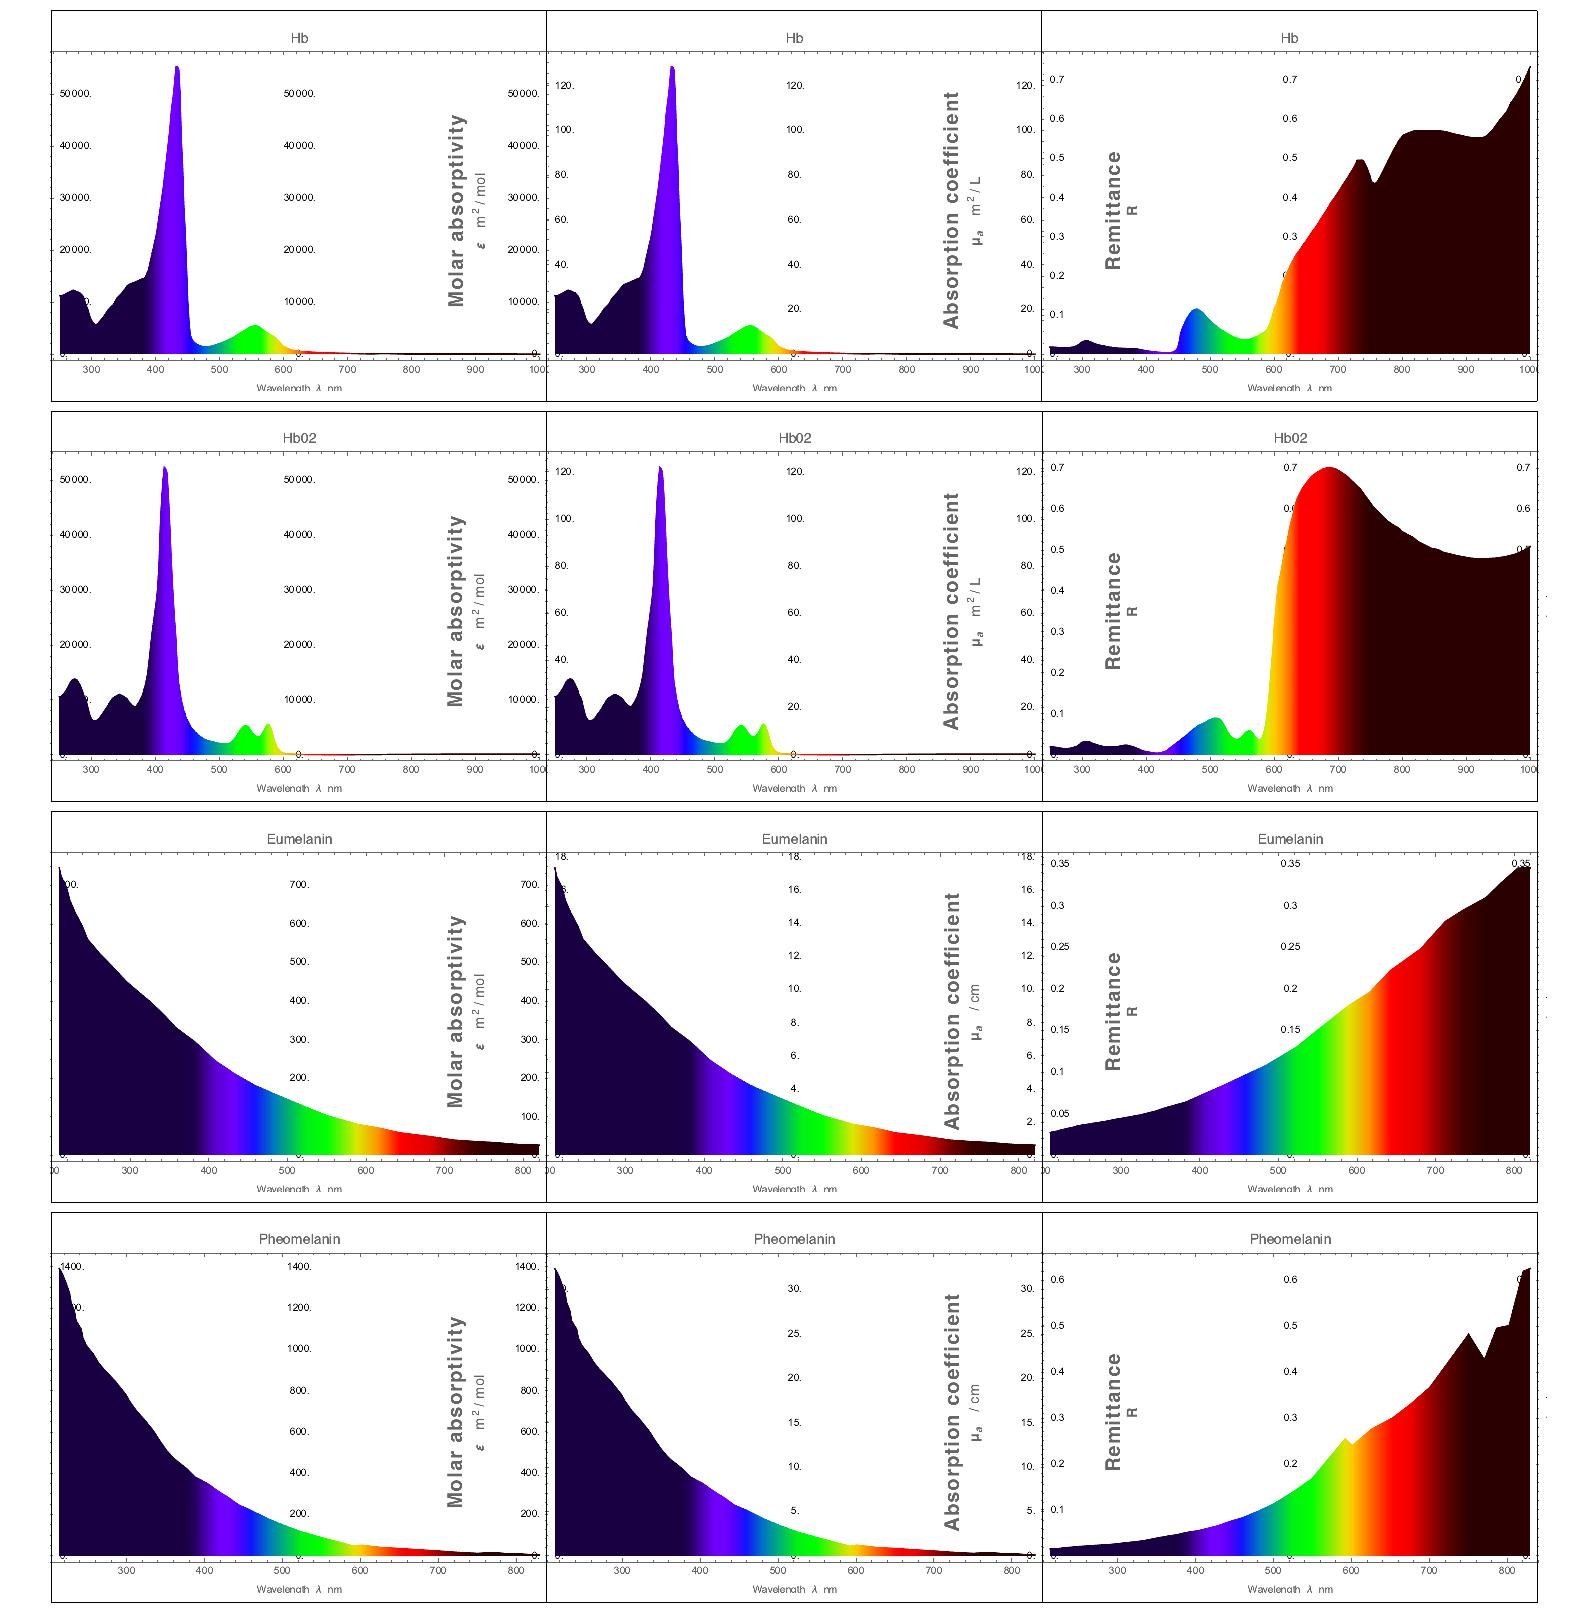
\includegraphics[width=0.99\textwidth]{Chapter1/Figs/ChemicalSpectralProperties.jpg}
    \caption{From left to right, the molar absorptivity, the absorption coefficient, and remittance of the four key chromophores. We assume a typical hemoglobin concentration of 150 $g/L$. The remittance was found using Kubelka-Munk Theory, outlined in section \ref{sec:SkinColorSimulation}. }  \label{fig:ChemicalSpectralProperties}
\end{figure}

The remittance spectra for the four key chromophores is shown in Figure \ref{fig:ChemicalSpectralProperties}. 

\subsection{Response Spectra}

The response spectrum is how a given sensor --- such as the human eye or a CCD --- responds to very specific wavelengths of light. Essentially, it is the raw output from the sensor. This is almost never used, and is generally inaccessible even at the hardware layer, as the circuitry very close to the CCD does a basic level of color rebalancing. As we don't know the full color correction for every possible CCD, we observed the raw output spectra of several different devices and then tried two very simple methods of rebalancing the color:

The first is peak normalization, which simply levels out the maximum output in each channel such that the peak output for each of the channels is equal. This approach is very simple, and is quite likely from an electrical engineering perspective as it facilitates the digitization of the color information.

The second method is to approach the response spectra as the basis functions for representing the spectrum. Using this approach, each basis function is normalized according to its integral over the visible wavelengths, giving an equal weighting to each of the response spectra functions over the range of values, rather than focusing on a peak value. Mathematically speaking, this approach is not unusual when constructing a basis set as it facilitates the maths.





It should be noted that the color balancing methods used in modern CCD devices are much more sophisticated than either of these approaches.

However, because the methods chosen here are straightforward amplifications of each channel, they're likely to be used as a first step in color rebalancing at the hardware level in the device. While we are not concerned with device constructions, it is useful to know how these devices capture the color information if this algorithm is to be used diagnostically, as color rebalancing may introduce artefacts and distortions in the data.

Although we consider these sensors to be capturing information throughout the entire visible spectrum, what they are actually capturing varies quite significantly between devices, as shown in Figure \ref{fig:ResponseSpectraStripes}. Even a very simple color rebalancing can restore some normality to the spectrum, as shown in Figure \ref{fig:ResponseSpectraStripesNorm}. However, as these devices use the aforementioned color rebalancing algorithms to alter the image to look more sensible to human eyes, these differences aren't so apparent to us.

\clearpage

\begin{figure}[h!]
  \centering
    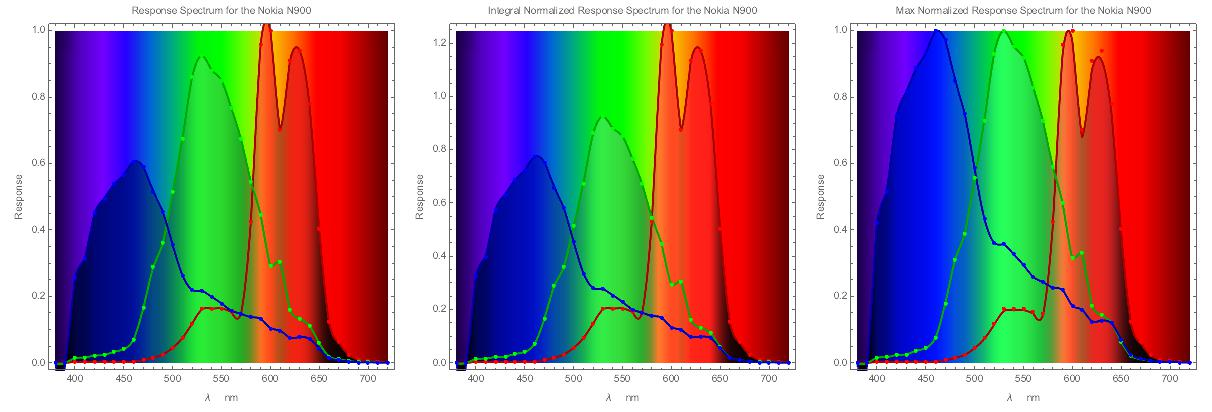
\includegraphics[width=0.99\textwidth]{Chapter1/Figs/ResponseSpectrum_NokiaN900.jpg}
    \caption{The response spectrum for the Nokia N900. }  \label{fig:ResponseSpectumNokia}
\end{figure}

\begin{figure}[h!]
  \centering
    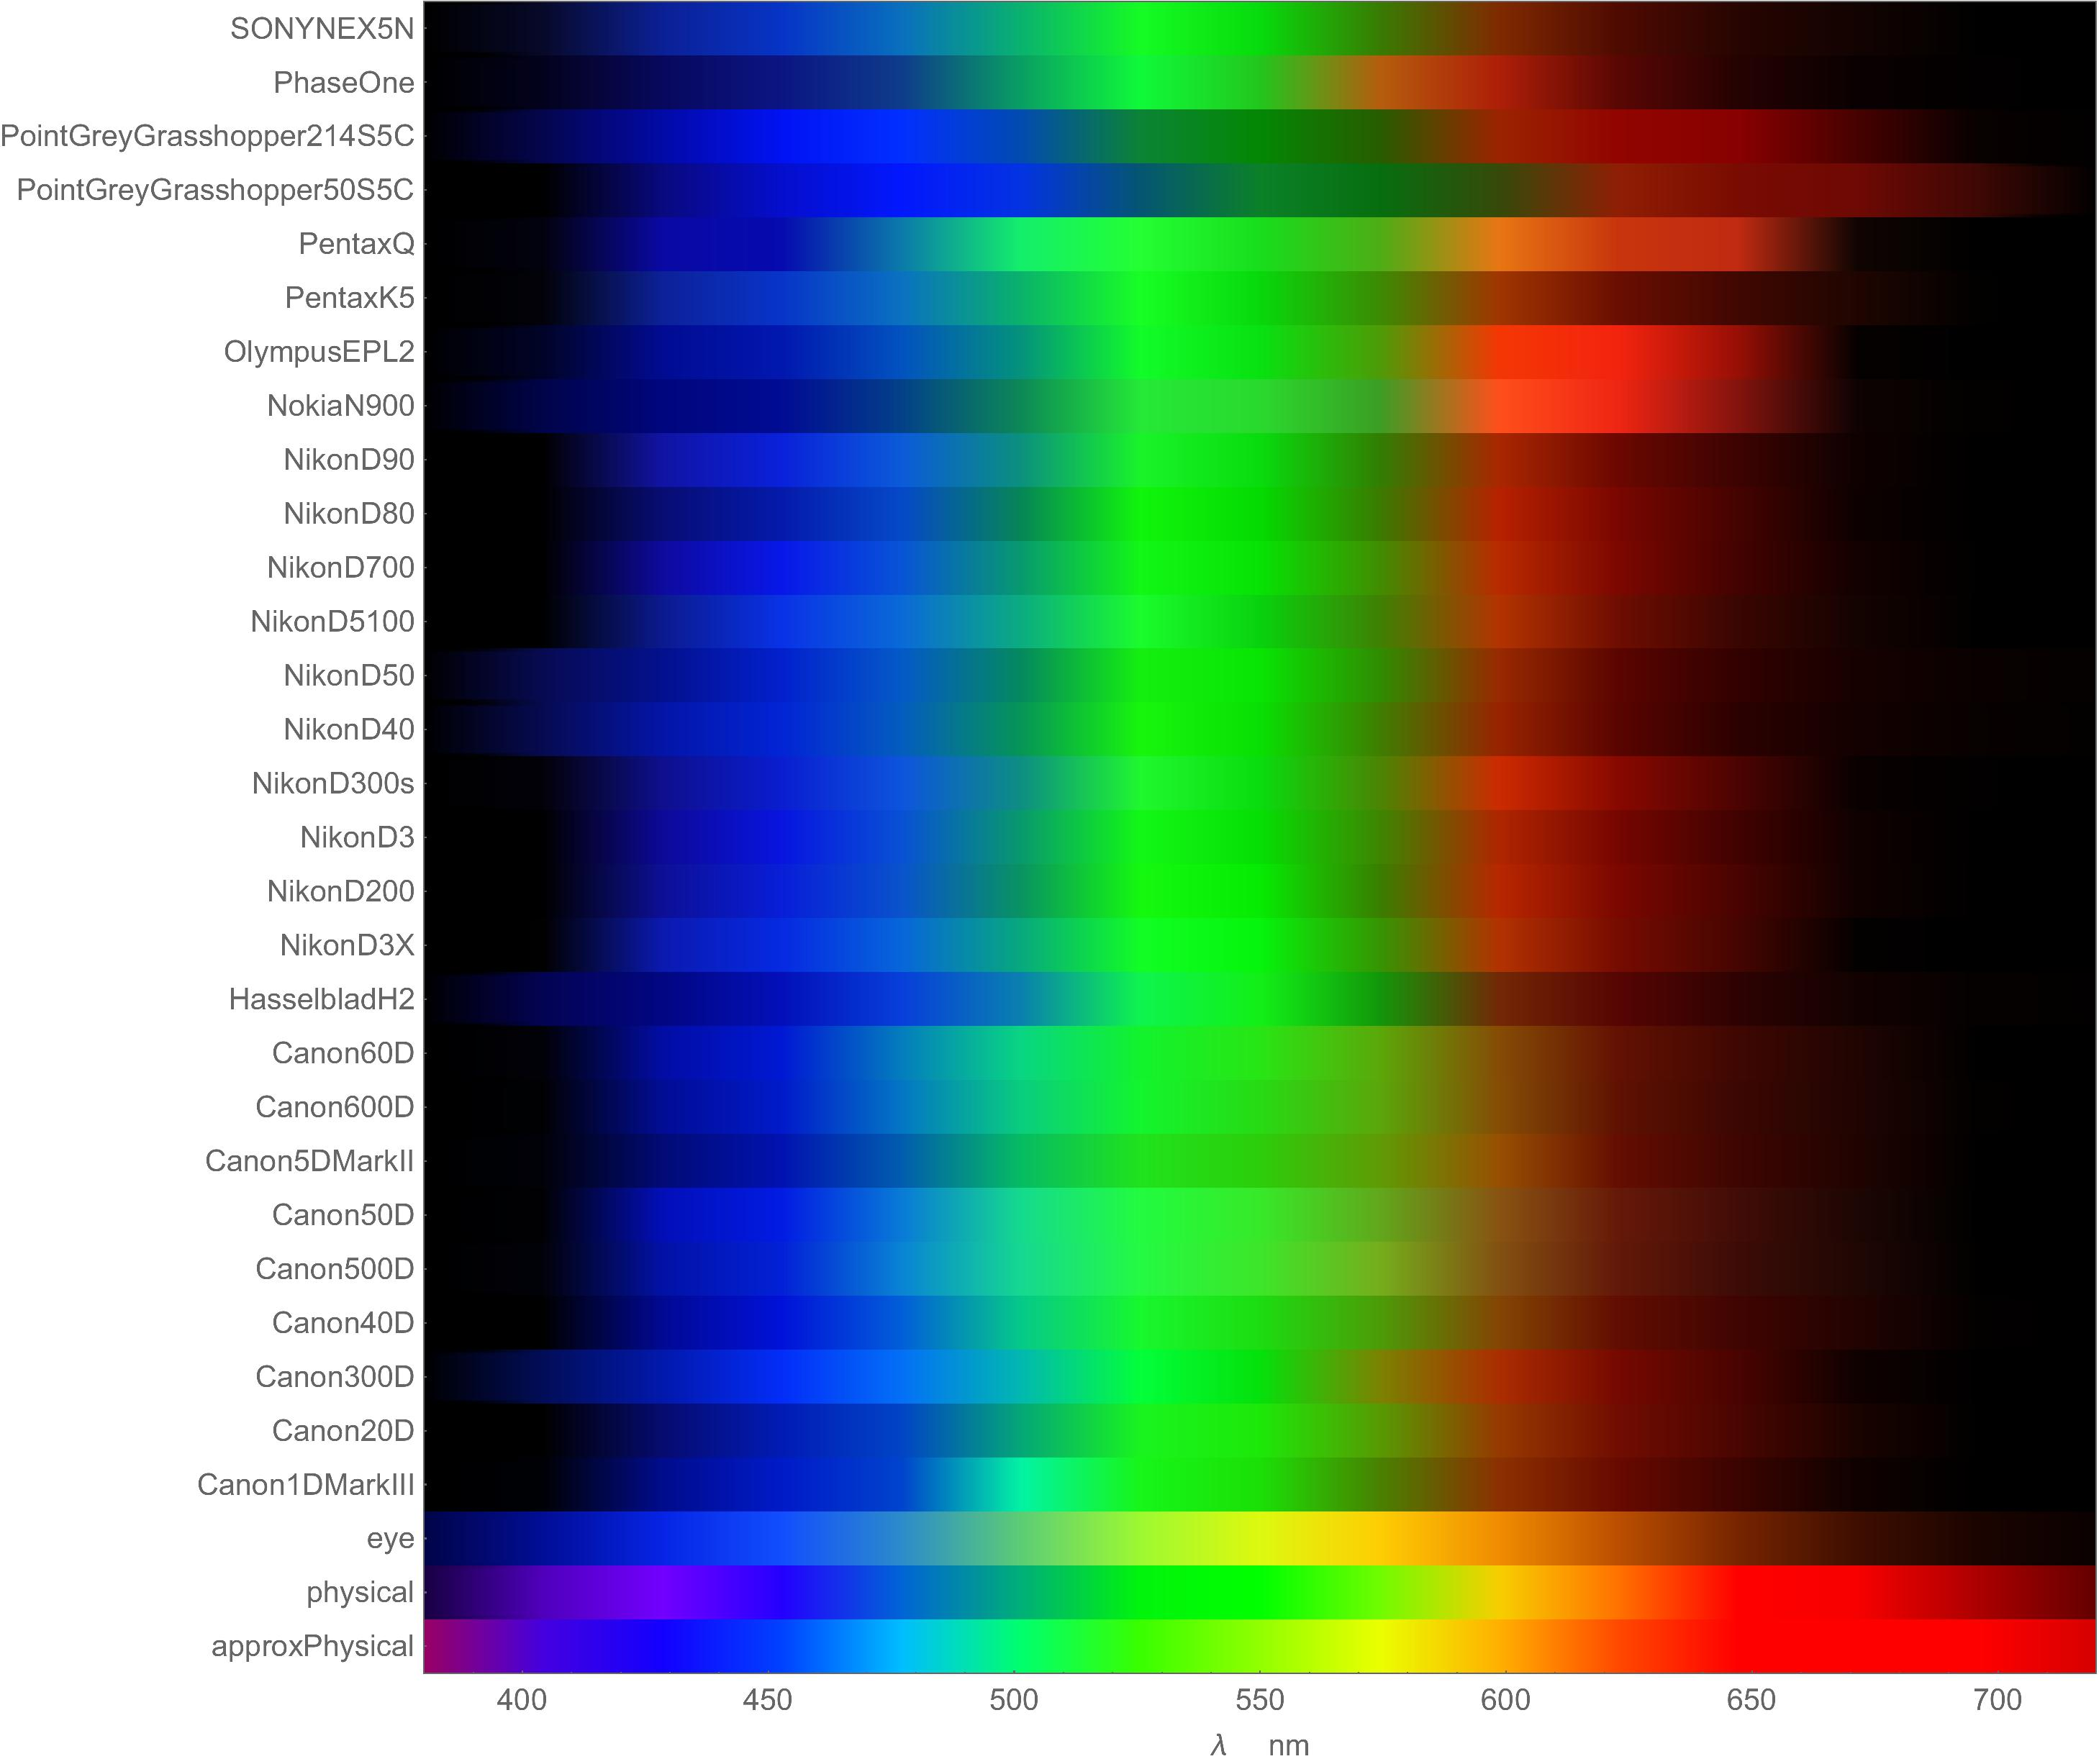
\includegraphics[width=0.99\textwidth]{Chapter1/Figs/ResponseSpectraStripes.jpg}
    \caption{The light spectrum as viewed using various CCDs with a physical spectrum for comparison.}  \label{fig:ResponseSpectraStripes}
\end{figure}

\clearpage

\begin{figure}[h!]
  \centering
    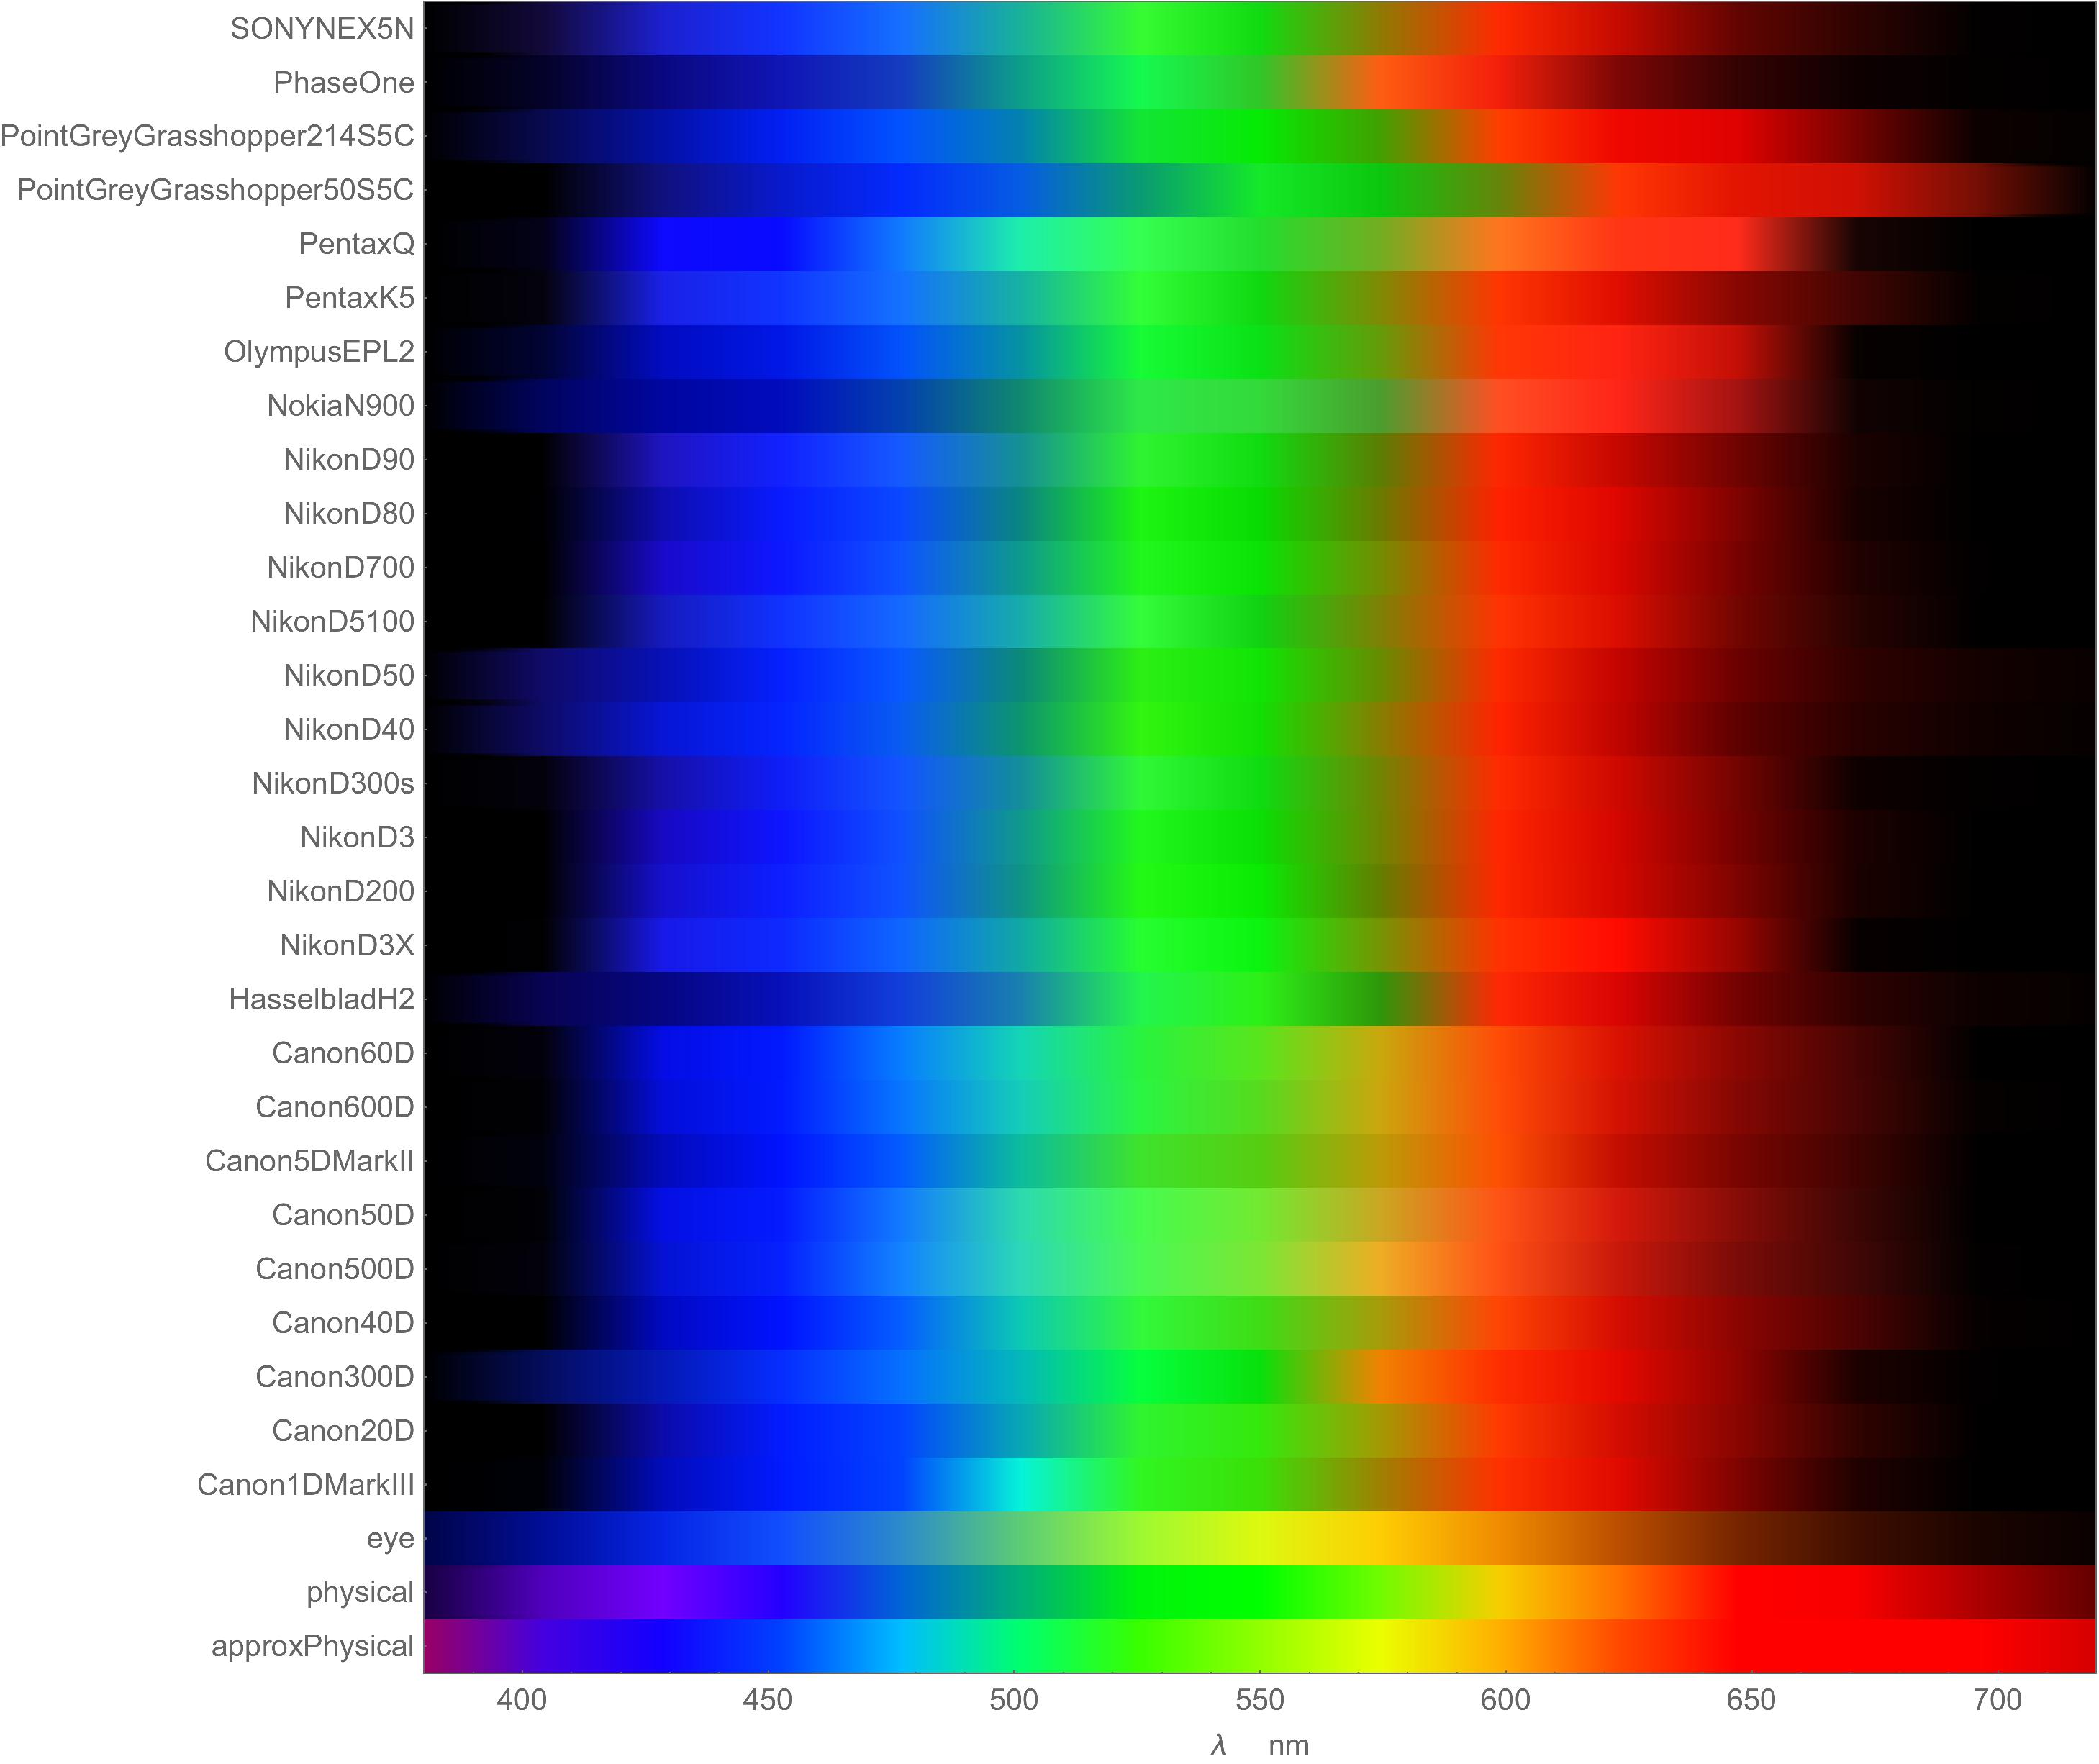
\includegraphics[width=0.99\textwidth]{Chapter1/Figs/ResponseSpectraStripesNorm.jpg}
    \caption{The light spectrum as viewed using various CCDs after normalization with a physical spectrum for comparison.}  \label{fig:ResponseSpectraStripesNorm}
\end{figure}

In addition to the color rebalancing, which corrects the behavior of the CCD devices, as is found in later sections, some devices, like the iPhone, also apply a dynamic color rebalancing which attempts to even out the colors based on the image captured. This feature is intended to correct for strange lighting conditions and other such problems which could affect the image. This will be addressed in detail in Chapter \ref{sec:Chap2}.

\clearpage

\subsection{Skin Color Simulation} \label{sec:SkinColorSimulation}

So, we have the molar absorptivity for the four key chromophores in the skin, we have the response spectra for a variety of devices, and a response spectra which serves as a target color output for all the devices after the color correction has been applied. Additionally, we are using the CIE 1931 RGB color space for the absorption spectra, which is closer to how our eyes perceive color than any other color space (\cite{RIDI2013}). This means that, in principle, we can get appropriate RGB values for the four key chromophores at the hardware layer using the device response spectra, or at the AP layer using the CIE 1931 RGB color space spectrum, assuming the device's color space correction does its job. The question now is how to actually simulate skin color.

Given a remittance spectrum $R(\lambda)$ and a response function $S_{rgb}(\lambda)$ for the sensor, the RGB output values can be calculated by finding the convolution 

\begin{align}
R & = \int_{0}^{\infty} R(\lambda) S_{R} (\lambda)  \mathbf{d\lambda}\\
G & = \int_{0}^{\infty} R(\lambda) S_{G} (\lambda) \mathbf{d\lambda}\\
B & = \int_{0}^{\infty} R(\lambda) S_{B} (\lambda)  \mathbf{d\lambda}
\end{align}

As for finding the RGB values, the bright color is the response of the CCD. By integrating the following functions in the figure below, we get the channel output seen in Figure~\ref{fig:Chromophores_NokiaN900}.


\begin{figure}[h!]
  \centering
    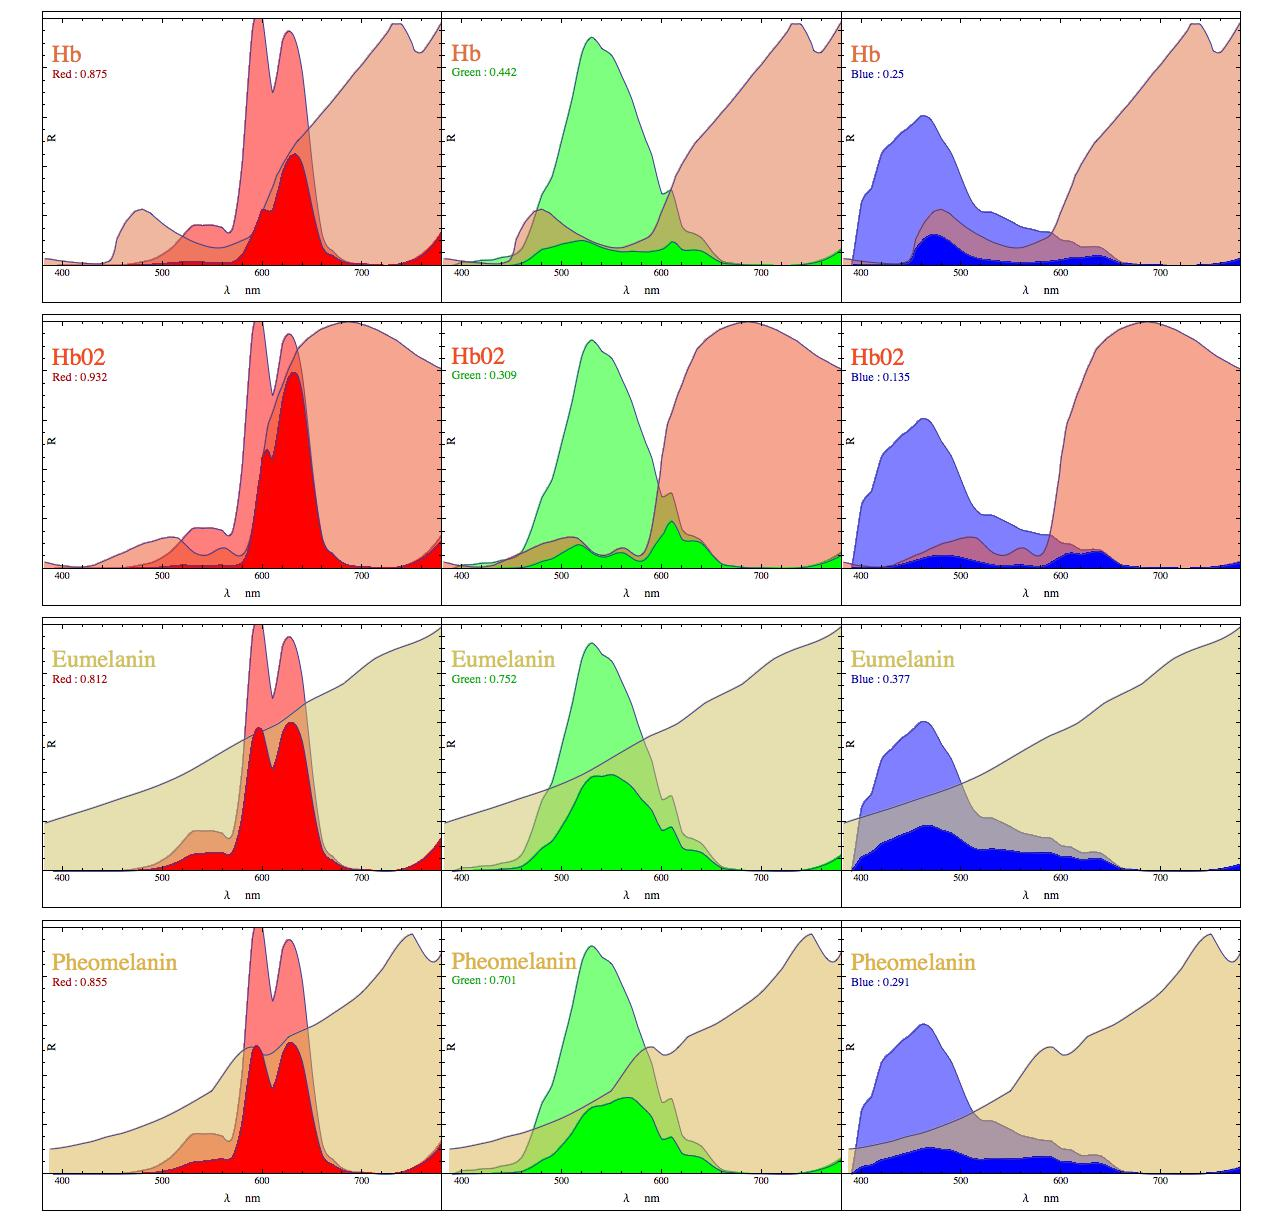
\includegraphics[width=0.99\textwidth]{Chapter1/Figs/Chromophores_NokiaN900.jpg}
    \caption{The functions representing the channel output of the four chromophores. The color of the remittance curve is the color for that particular chromophore as seen by the NokiaN900 camera. The solid-filled, bright function is the response of the CCD for each of the channels to that limited light, and the pale function is the response function of the CCD for each of the channels.}  \label{fig:Chromophores_NokiaN900}
\end{figure}



Thus, we can now find the channel output of any device for which we have a response function (Figure \ref{fig:CameraComparison}).

At the time of development, access to the camera on the iPhone was limited to the AP layer, and so we work with the CIE 1931 RGB color space. The relative position of the chromophores in the chromatic space, i.e. a color space with a luminosity axis, is shown in Figure \ref{fig:ChromophoresYAB}.



%********************************** %First Section  **************************************
%\section{Motivation} %Section - 1.1 





%********************************** %Second Section  *************************************
%\section{Overview of Color Spaces} %Section - 1.2


%********************************** % Third Section  *************************************
%\section{Where does it come from?}  %Section - 1.3 
%\label{section1.3}


\begin{figure}[h!] %hi-res
  \centering
    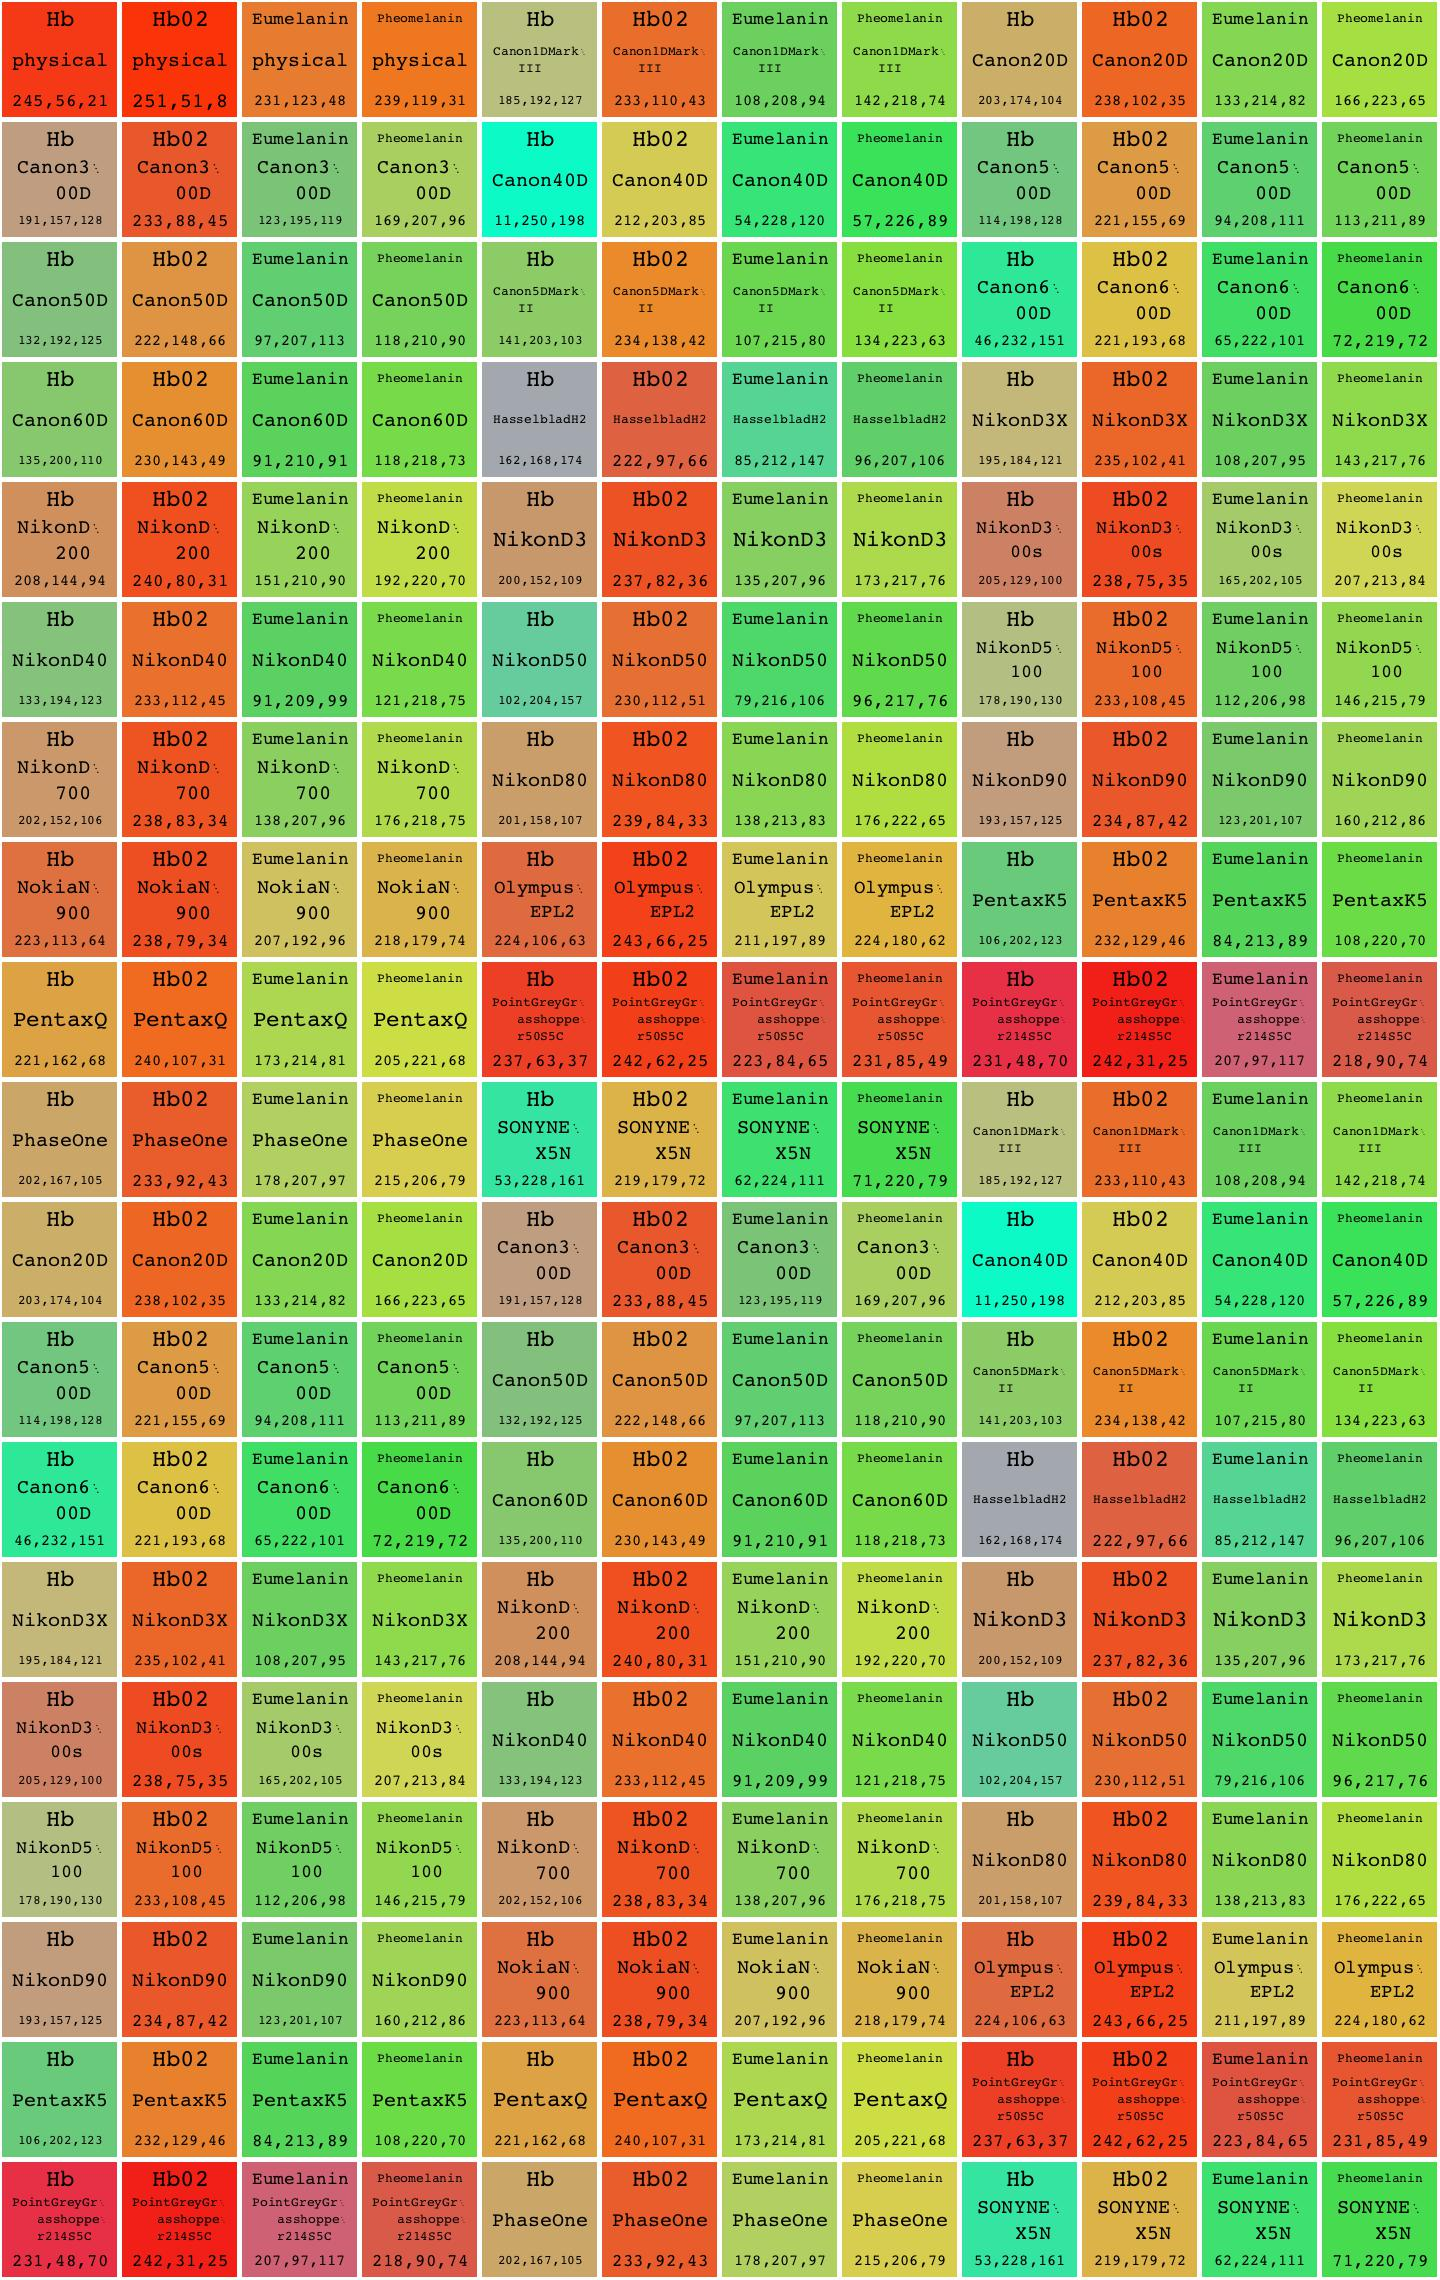
\includegraphics[width=0.99\textwidth]{Chapter1/Figs/CameraComparison.jpg}
    \caption{Chromophore colors as perceived by a range of devices.}  \label{fig:CameraComparison}
\end{figure}

\begin{figure}[h!]
  \centering
    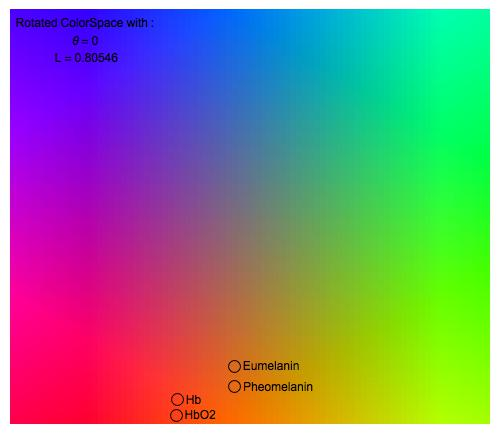
\includegraphics[width=0.99\textwidth]{Chapter1/Figs/ChromophoresYAB.jpg}
    \caption{The four main chromophores as perceived by CIE 1931 RGB color space after rotation into the LCaCb $\theta = 0$ color space.}  \label{fig:ChromophoresYAB}
\end{figure}